% ==========================================
% 3. Questão 3
% (o título da seção e o \addcontentsline ficam no homework1.tex;
%  este arquivo é incluído logo abaixo deles com % ==========================================
% 3. Questão 3
% (o título da seção e o \addcontentsline ficam no homework1.tex;
%  este arquivo é incluído logo abaixo deles com % ==========================================
% 3. Questão 3
% (o título da seção e o \addcontentsline ficam no homework1.tex;
%  este arquivo é incluído logo abaixo deles com % ==========================================
% 3. Questão 3
% (o título da seção e o \addcontentsline ficam no homework1.tex;
%  este arquivo é incluído logo abaixo deles com \input{questao3})
% ==========================================

A questão 3 solicita o uso da variável \texttt{low\_usage} previamente definida na questão 2 para investigar as características associadas aos dias de menor uso do sistema.

% ==========================================
% 3.0 Definições
% ==========================================

\subsection*{Definições}
\addcontentsline{toc}{subsection}{Definições}
\noindent \textit{def} - Desvio padrão: indica o quão espalhados estão os valores de um conjunto de dados em relação à média, utilizado aqui como desvio padrão amostral, já que estamos analisando uma amostra de 300 valores de uma população total de 731. O desvio padrão amostral é o mesmo utilizado pela função \texttt{sd()} do R, dado pela fórmula:

\begin{equation*}
    s = \sqrt{\frac{1}{N-1}\sum_{i=1}^{N}\left(x_i-\overline{x}\right)^2}
\end{equation*}

\noindent \textit{def} - Coeficiente de correlação de Pearson: mede a intensidade da relação linear entre duas variáveis quantitativas, retornando um valor entre $-1$ e $1$, dado pela fórmula:

\begin{equation*}
    r = \frac{\sum\left(x_i-\overline{x}\right)\left(y_i-\overline{y}\right)}{\sqrt{\sum\left(x_i-\overline{x}\right)^2\sum\left(y_i-\overline{y}\right)^2}}
\end{equation*}

% ==========================================
% 3.1 Item 1
% ==========================================

\subsection*{Item 1}
\addcontentsline{toc}{subsection}{Item 1}
Este item pede para calcular média, mediana e desvio padrão de \texttt{total\_user} para cada estação do ano e determinar a proporção de dias classificados como \texttt{low\_usage} e, além disso, construir um boxplot comparando cada estação.

Para a resolução do item 1, segue o código em R e a explicação de cada trecho:

% ----------- Código 11 -------------
\begin{rcode}[firstnumber=109, caption={Análise da utilização do sistema em cada estação do ano},breaklines=true, breakatwhitespace=true]
    # Questão 3
    # Item 1
    # Convertendo season numérico para categórico
    data_group$season <- factor(data_group$season,
                                levels = c(1, 2, 3, 4),
                                labels = c("Inverno", "Primavera", "Verão", "Outono"))
    # Média de usuários por estação do ano
    tapply(total_user, data_group$season, mean)
    # Mediana de usuários por estação
    tapply(total_user, data_group$season, median)
    # Desvio padrão de total_user por estação
    tapply(total_user, data_group$season, sd)
    # Proporção de dias classificados como low_usage por estação
    tapply(low_usage, data_group$season, mean)

    boxplot(total_user ~ data_group$season,
            main = "Comparação do uso do sistema por Estação", #Titulo
            xlab = "Estação do Ano", #legenda eixo x
            ylab = "Total de Usuários", #legenda eixo y
            medcol = "#D32F2F",        # Cor da mediana
            col = c("#81C784", "#FFF176", "#FFB74D", "#64B5F6"), #cores das caixas
            border = "#2E7D32") #cor da borda da caixa
\end{rcode}

Primeiro é feita a conversão da variável \texttt{season} de numérica para categórica usando \texttt{factor} para associar o nome de cada estação ao seu respectivo número (1, 2, 3, 4). A conversão não altera os valores calculados, apenas faz com que os grupos sejam identificados pelo nome da estação, tanto na saída da função \texttt{tapply} quanto no eixo do boxplot. Depois, é utilizada a função \texttt{tapply()} para dividir o vetor de \texttt{total\_user} em subgrupos, um para cada estação do ano, e aplicar uma função (no caso aqui, as funções de média, mediana e desvio padrão) a cada subgrupo deste vetor. O resultado obtido no R está na tabela a seguir:

% ----------- Tabela 7  -------------
\begin{table}[h!]
    \centering
    \caption{Resultados para cada estação}
    \label{tab:mascara_7u}
    \begin{tabular}{c|c|c|c|c}
        Medição & Inverno & Primavera & Verão & Outono \\\hline
        Média &2000.76 &3775.17 &4464.36 &3664.46 \\ \hline
        Mediana &2077.00 &4085.50 &4615.50 &3717.00 \\ \hline
        Desvio padrão &738.80 &1138.90 &798.35 &983.01 \\ \hline
        Proporção (\texttt{low\_usage}) &0.92 &0.26 &0.04 &0.27
    \end{tabular}
\end{table}

Como a variável \texttt{low\_usage} é 0 ou 1, fazer a média retorna exatamente a proporção, já que estamos somando os dias classificados como \texttt{low\_usage} e dividindo pela quantidade de dias.

Para a construção do boxplot, foi feita a criação do gráfico fazendo:
\begin{center}
    \texttt{total\_user \textasciitilde{} data\_group\$season}
\end{center}
Ou seja, \texttt{total\_user} em função da variável \texttt{season}, gerando uma caixa para cada estação. O boxplot gerado está exibido a seguir:

% ------------ Imagem 3 -----------
\begin{figure}[htbp]
    \centering
    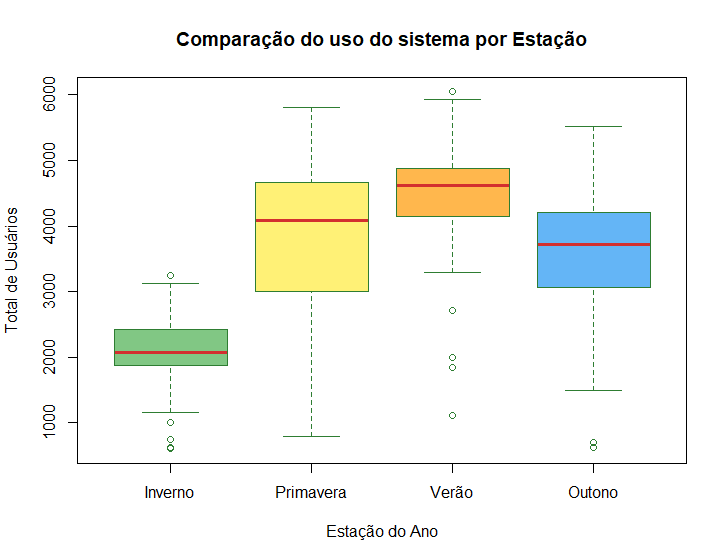
\includegraphics[width=0.6\textwidth]{Boxplot_estacoes.png}
    \caption{Boxplot do total de usuários por estação}
    \label{fig:boxplot_estacoes}
\end{figure}

Os resultados evidenciam uma clara associação entre as estações do ano e o uso do sistema, mostrando que o uso diminui consideravelmente no período de inverno e aumenta nas estações mais quentes. Além disso, a extração da proporção de dias classificados como \texttt{low\_usage} denota que a grande maioria dos dias de inverno é classificada como de baixa utilização do sistema, ademais, o uso do sistema no verão aumenta mais que o dobro do que no inverno, com o verão tendo uma média total de usuários do sistema de 4464.36 contra uma média de 2000.76 usuários no inverno. Outra informação relevante é que as estações de primavera e outono possuem média de usuários diária bem próxima, o que demonstra que o uso do sistema é bem equivalente entre essas duas estações, com uma ressalva de que a primavera tem alto desvio padrão comparado às outras estações, evidenciando uma notável disparidade entre dias de maior uso e de menor uso dentro da própria estação devido a fatores além da estação do ano.

% ==========================================
% 3.2 Item 2
% ==========================================

\subsection*{Item 2}
\addcontentsline{toc}{subsection}{Item 2}
Este item busca investigar a relação do uso do sistema em função das condições meteorológicas. Para isso, o item pede que, para cada condição, seja calculada a média e o desvio padrão de \texttt{total\_user} e determinada a proporção de dias classificados como \texttt{low\_usage}.

Para isso, foi utilizado o seguinte código em R:

% ----------- Código 12 -------------
\begin{rcode}[firstnumber=132, caption={Análise da utilização do sistema para cada condição meteorológica},breaklines=true, breakatwhitespace=true]
    # Item 2
    # Convertendo weathersit de numérico para categórico
    data_group$weathersit <- factor(data_group$weathersit,
                                    levels = c(1, 2, 3, 4),
                                    labels = c("Céu limpo", "Nublado", "Chuva fraca", "Chuva forte"))

    # Média total_user por condição meteorológica
    tapply(total_user, data_group$weathersit, mean)

    # Desvio padrão de total_user por condição meteorológica
    tapply(total_user, data_group$weathersit, sd)

    # Proporção de dias de baixa utilização (low_usage) por condição meteorológica
    tapply(low_usage, data_group$weathersit, mean)
\end{rcode}

Assim como na resolução do item 1, foi utilizada a seguinte linha de raciocínio: para cada valor correspondente a determinada condição climática constatada no \texttt{data\_group}, foi associado o nome correspondente da condição climática utilizando \texttt{factor}, para facilitar a identificação e interpretação dos dados tanto nos resultados da função \texttt{tapply} quanto em representações gráficas. Após isso, usando a função \texttt{tapply} para aplicar as funções de média e desvio padrão a cada subgrupo de \texttt{total\_user} e de \texttt{low\_usage} (um para cada condição meteorológica), obtiveram-se os seguintes resultados de média, desvio padrão e proporção de dias classificados como baixo uso do sistema, constatados na tabela a seguir:

% ----------- Tabela 8  -------------
\begin{table}[h!]
    \centering
    \caption{Resultados para cada condição meteorológica}
    \label{tab:mascara_8u}
    \begin{tabular}{c|c|c|c|c}
        Medição & Céu limpo & Nublado & Chuva fraca & Chuva forte \\\hline
        Média &4159.22 &3462.94 &1757.57 &-- \\ \hline
        Desvio padrão &984.66 &1090.92 &793.95 &-- \\ \hline
        Proporção (\texttt{low\_usage}) &0.14 &0.35 &1.00 &--
    \end{tabular}
\end{table}

Analisando os resultados, nota-se de imediato duas informações cruciais: não se obtiveram dados para a categoria de chuva forte, pois o \texttt{data\_group} de 300 amostras não possui dias classificados meteorologicamente com essa condição climática; além disso, destaca-se a proporção de dias de baixo uso igual a 1, ou seja, nos dias de chuva fraca da amostra, o total de usuários ficou sempre abaixo do primeiro quartil (Q1) definido para a amostra inteira.

Para realizar uma comparação visual entre as condições meteorológicas, usou-se também um gráfico construído a partir do seguinte código em R:

% ----------- Código 13 -------------
\begin{rcode}[firstnumber=147, caption={Construção de boxplot para análise da utilização do sistema para cada condição meteorológica},breaklines=true, breakatwhitespace=true]
    # Boxplot
    boxplot(total_user ~ data_group$weathersit,
            main = "Utilização do Sistema por Condição Meteorológica",
            xlab = "Condições Meteorológicas",
            ylab = "Total de Usuários",
            col = c("#FFF176", "#D3D3D3", "#00A8FF", "#173A59"),
            border = "#2E7D32")
\end{rcode}

% ------------ Imagem 4 -----------
\begin{figure}[htbp]
    \centering
    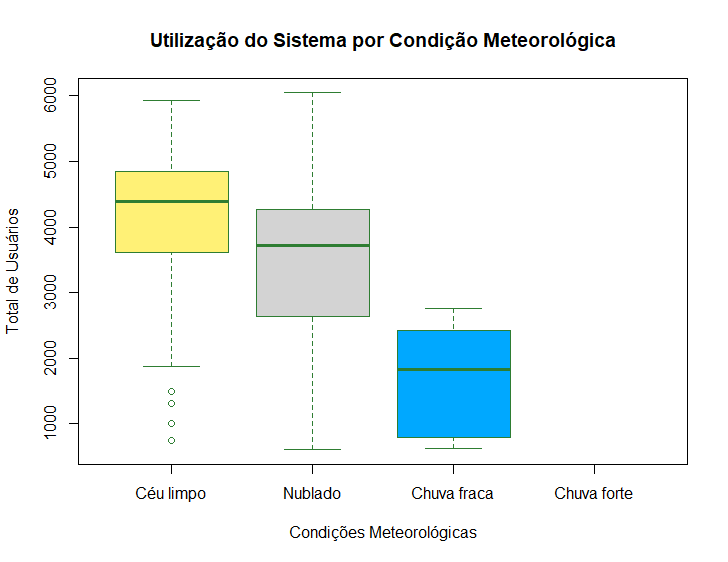
\includegraphics[width=0.6\textwidth]{Boxplot_clima.png}
    \caption{Boxplot do total de usuários por condição meteorológica}
    \label{fig:boxplot_clima}
\end{figure}

Os resultados indicam que a demanda pelo sistema cai de forma expressiva à medida que as condições meteorológicas se deterioram. A média de usuários cai de cerca de 4159, em dias de céu limpo, para apenas 1757, em dias de chuva fraca, o que corresponde a quase 2/3 a menos de usuários do sistema em dias de chuva fraca em comparação com o céu limpo, o que se nota graficamente pela queda em \textquotedblleft degraus\textquotedblright{} das medianas representadas no boxplot. Além disso, observa-se uma imprevisibilidade no uso do sistema em dias nublados, tanto pelo maior desvio padrão quanto pelo tamanho da caixa e dos bigodes no boxplot, mostrando que, mesmo com o clima nublado, há dias de uso bastante elevado do sistema, enquanto outros igualam o nível de uso em dias chuvosos, denotando a clara variabilidade no comportamento dos usuários frente a essa condição climática.

% ==========================================
% 3.3 Item 3
% ==========================================

\subsection*{Item 3}
\addcontentsline{toc}{subsection}{Item 3}
Este item busca investigar a relação entre temperatura e \texttt{total\_user}, usando para isso um gráfico de dispersão e o coeficiente de correlação para descrever a relação observada. Para isso, foi utilizado o seguinte código em R:

% ----------- Código 14 -------------
\begin{rcode}[firstnumber=155, caption={Obtenção do coeficiente de correlação de Pearson e plotagem do gráfico de dispersão},breaklines=true, breakatwhitespace=true]
    #item 3
    # Cálculo do coeficiente de correlação de Pearson
    correlacao <- cor(data_group$temp, total_user)
    print(correlacao)

    # Construção do gráfico de dispersão
    plot(data_group$temp, total_user,
        main = "Relação entre temperatura e utilização do sistema",
        xlab = "Temperatura em graus Celsius",
        ylab = "Total de Usuários",
        pch = 19,               # Formato do ponto (bolinha preenchida)
        col = "#2E7D32",        # Cor dos pontos
        frame.plot = FALSE)     # Remove a moldura externa superior e direita
\end{rcode}

Primeiro é extraído diretamente o coeficiente de correlação (que no R, por padrão, é o de Pearson) através da função \texttt{cor(data\_group\$temp, total\_user)}, correlacionando a temperatura e o \texttt{total\_user}.

O resultado obtido no terminal foi $r = 0.6386851$, o que denota uma correlação positiva e moderada-alta, ainda distante de 1, o que indica que, com o aumento da temperatura, o número de usuários do sistema tende a aumentar, entretanto com uma considerável dispersão dos pontos no gráfico, indicando que outros fatores também influenciam nessa relação.

% ------------ Imagem 5 -----------
\begin{figure}[htbp]
    \centering
    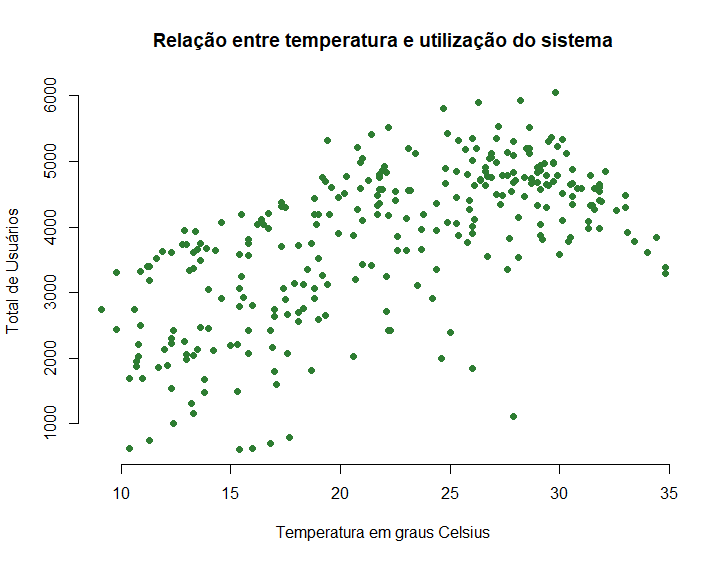
\includegraphics[width=0.55\textwidth]{Dispersao_temp.png}
    \caption{Gráfico de dispersão (\texttt{total\_user} x temperatura)}
    \label{fig:dispersao_temp}
\end{figure}

Evidenciam-se, portanto, algumas limitações do coeficiente de Pearson para descrever essa relação. Por exemplo, o $r$ de Pearson é estritamente linear, o que reduz sua precisão em relações não lineares: nota-se um crescimento quase linear até por volta dos 30°C, e depois disso o total de usuários começa a cair com o aumento da temperatura, o que formaria uma curva em parábola, relação que o coeficiente linear não captura. Além disso, por natureza, correlação não implica causalidade, e também é sensível a outliers, como pontos isolados de baixo uso do sistema bem abaixo do padrão da vizinhança, que tende a ser mais alto.

% ==========================================
% 3.4 Item 4
% ==========================================

\subsection*{Item 4}
\addcontentsline{toc}{subsection}{Item 4}
Este item pede para escolher 2 das 3 categorias analisadas previamente nesta questão que parecem estar mais associadas à utilização do sistema. Baseado nos dados obtidos e na análise feita, as duas categorias escolhidas serão a condição meteorológica e a temperatura, pois, apesar da estação do ano influenciar a demanda do sistema, ela é uma categoria que engloba em partes características das outras duas. Por exemplo, no item 1 observou-se que, no inverno, a demanda pelo sistema cai consideravelmente; entretanto, o inverno afasta as pessoas justamente pelo fato de ter temperaturas baixas e condições meteorológicas mais turbulentas, e nos itens 2 e 3 foi comprovado que condições meteorológicas piores e temperaturas baixas têm, no geral, baixa adesão dos usuários ao sistema. Feita essa escolha das 2 categorias, os resultados estatísticos mostram o seguinte sobre elas:

\textit{Condições meteorológicas:}

Observou-se que esta categoria é um fator altamente impactante na demanda do sistema, visto que a média de usuários despencou de 4159, em dias de céu limpo, para somente 1757, em dias de chuva fraca. Além disso, através da análise da proporção de dias classificados como \texttt{low\_usage}, 100\% dos dias com chuva fraca registraram baixa utilização do sistema, provando ser um fator drástico que limita a quantidade de usuários que aderem ao sistema de aluguel de bicicletas, sendo assim uma categoria intensamente associada à utilização do sistema.

\textit{Temperatura:}

Os resultados mostram que a temperatura possui considerável relação com a utilização do sistema. Através do coeficiente de correlação de Pearson obtido ($r \approx 0.64$), evidencia-se uma forte associação linear positiva, com o gráfico de dispersão ilustrando claramente o aumento gradual no número de usuários conforme a temperatura aumenta, até um limite de conforto e saúde por volta de 30-32°C. Além disso, o gráfico de dispersão, apesar de estar analisando a relação temperatura x total de usuários, também reforça a associação encontrada no item 1 entre estação do ano e \texttt{total\_user}, constatando-se que estações do ano mais frias apresentam médias de usuários menores do que estações mais quentes, com a média de usuários do inverno (2000) sendo menos da metade da média de usuários do verão (4464).
)
% ==========================================

A questão 3 solicita o uso da variável \texttt{low\_usage} previamente definida na questão 2 para investigar as características associadas aos dias de menor uso do sistema.

% ==========================================
% 3.0 Definições
% ==========================================

\subsection*{Definições}
\addcontentsline{toc}{subsection}{Definições}
\noindent \textit{def} - Desvio padrão: indica o quão espalhados estão os valores de um conjunto de dados em relação à média, utilizado aqui como desvio padrão amostral, já que estamos analisando uma amostra de 300 valores de uma população total de 731. O desvio padrão amostral é o mesmo utilizado pela função \texttt{sd()} do R, dado pela fórmula:

\begin{equation*}
    s = \sqrt{\frac{1}{N-1}\sum_{i=1}^{N}\left(x_i-\overline{x}\right)^2}
\end{equation*}

\noindent \textit{def} - Coeficiente de correlação de Pearson: mede a intensidade da relação linear entre duas variáveis quantitativas, retornando um valor entre $-1$ e $1$, dado pela fórmula:

\begin{equation*}
    r = \frac{\sum\left(x_i-\overline{x}\right)\left(y_i-\overline{y}\right)}{\sqrt{\sum\left(x_i-\overline{x}\right)^2\sum\left(y_i-\overline{y}\right)^2}}
\end{equation*}

% ==========================================
% 3.1 Item 1
% ==========================================

\subsection*{Item 1}
\addcontentsline{toc}{subsection}{Item 1}
Este item pede para calcular média, mediana e desvio padrão de \texttt{total\_user} para cada estação do ano e determinar a proporção de dias classificados como \texttt{low\_usage} e, além disso, construir um boxplot comparando cada estação.

Para a resolução do item 1, segue o código em R e a explicação de cada trecho:

% ----------- Código 11 -------------
\begin{rcode}[firstnumber=109, caption={Análise da utilização do sistema em cada estação do ano},breaklines=true, breakatwhitespace=true]
    # Questão 3
    # Item 1
    # Convertendo season numérico para categórico
    data_group$season <- factor(data_group$season,
                                levels = c(1, 2, 3, 4),
                                labels = c("Inverno", "Primavera", "Verão", "Outono"))
    # Média de usuários por estação do ano
    tapply(total_user, data_group$season, mean)
    # Mediana de usuários por estação
    tapply(total_user, data_group$season, median)
    # Desvio padrão de total_user por estação
    tapply(total_user, data_group$season, sd)
    # Proporção de dias classificados como low_usage por estação
    tapply(low_usage, data_group$season, mean)

    boxplot(total_user ~ data_group$season,
            main = "Comparação do uso do sistema por Estação", #Titulo
            xlab = "Estação do Ano", #legenda eixo x
            ylab = "Total de Usuários", #legenda eixo y
            medcol = "#D32F2F",        # Cor da mediana
            col = c("#81C784", "#FFF176", "#FFB74D", "#64B5F6"), #cores das caixas
            border = "#2E7D32") #cor da borda da caixa
\end{rcode}

Primeiro é feita a conversão da variável \texttt{season} de numérica para categórica usando \texttt{factor} para associar o nome de cada estação ao seu respectivo número (1, 2, 3, 4). A conversão não altera os valores calculados, apenas faz com que os grupos sejam identificados pelo nome da estação, tanto na saída da função \texttt{tapply} quanto no eixo do boxplot. Depois, é utilizada a função \texttt{tapply()} para dividir o vetor de \texttt{total\_user} em subgrupos, um para cada estação do ano, e aplicar uma função (no caso aqui, as funções de média, mediana e desvio padrão) a cada subgrupo deste vetor. O resultado obtido no R está na tabela a seguir:

% ----------- Tabela 7  -------------
\begin{table}[h!]
    \centering
    \caption{Resultados para cada estação}
    \label{tab:mascara_7u}
    \begin{tabular}{c|c|c|c|c}
        Medição & Inverno & Primavera & Verão & Outono \\\hline
        Média &2000.76 &3775.17 &4464.36 &3664.46 \\ \hline
        Mediana &2077.00 &4085.50 &4615.50 &3717.00 \\ \hline
        Desvio padrão &738.80 &1138.90 &798.35 &983.01 \\ \hline
        Proporção (\texttt{low\_usage}) &0.92 &0.26 &0.04 &0.27
    \end{tabular}
\end{table}

Como a variável \texttt{low\_usage} é 0 ou 1, fazer a média retorna exatamente a proporção, já que estamos somando os dias classificados como \texttt{low\_usage} e dividindo pela quantidade de dias.

Para a construção do boxplot, foi feita a criação do gráfico fazendo:
\begin{center}
    \texttt{total\_user \textasciitilde{} data\_group\$season}
\end{center}
Ou seja, \texttt{total\_user} em função da variável \texttt{season}, gerando uma caixa para cada estação. O boxplot gerado está exibido a seguir:

% ------------ Imagem 3 -----------
\begin{figure}[htbp]
    \centering
    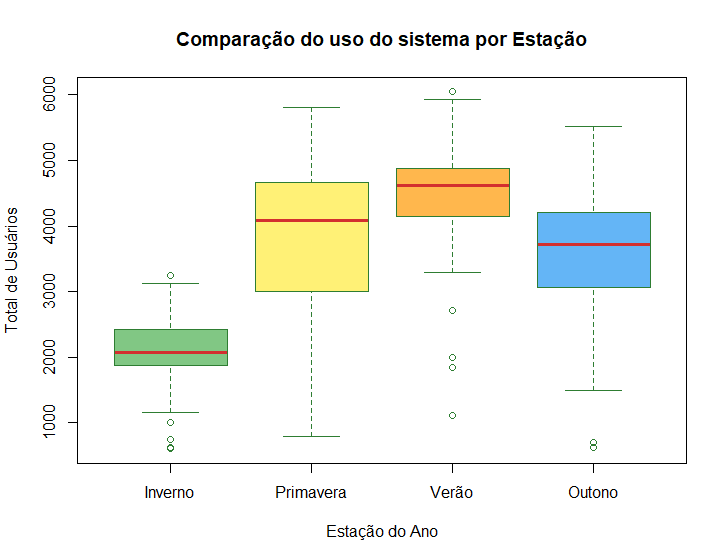
\includegraphics[width=0.6\textwidth]{Boxplot_estacoes.png}
    \caption{Boxplot do total de usuários por estação}
    \label{fig:boxplot_estacoes}
\end{figure}

Os resultados evidenciam uma clara associação entre as estações do ano e o uso do sistema, mostrando que o uso diminui consideravelmente no período de inverno e aumenta nas estações mais quentes. Além disso, a extração da proporção de dias classificados como \texttt{low\_usage} denota que a grande maioria dos dias de inverno é classificada como de baixa utilização do sistema, ademais, o uso do sistema no verão aumenta mais que o dobro do que no inverno, com o verão tendo uma média total de usuários do sistema de 4464.36 contra uma média de 2000.76 usuários no inverno. Outra informação relevante é que as estações de primavera e outono possuem média de usuários diária bem próxima, o que demonstra que o uso do sistema é bem equivalente entre essas duas estações, com uma ressalva de que a primavera tem alto desvio padrão comparado às outras estações, evidenciando uma notável disparidade entre dias de maior uso e de menor uso dentro da própria estação devido a fatores além da estação do ano.

% ==========================================
% 3.2 Item 2
% ==========================================

\subsection*{Item 2}
\addcontentsline{toc}{subsection}{Item 2}
Este item busca investigar a relação do uso do sistema em função das condições meteorológicas. Para isso, o item pede que, para cada condição, seja calculada a média e o desvio padrão de \texttt{total\_user} e determinada a proporção de dias classificados como \texttt{low\_usage}.

Para isso, foi utilizado o seguinte código em R:

% ----------- Código 12 -------------
\begin{rcode}[firstnumber=132, caption={Análise da utilização do sistema para cada condição meteorológica},breaklines=true, breakatwhitespace=true]
    # Item 2
    # Convertendo weathersit de numérico para categórico
    data_group$weathersit <- factor(data_group$weathersit,
                                    levels = c(1, 2, 3, 4),
                                    labels = c("Céu limpo", "Nublado", "Chuva fraca", "Chuva forte"))

    # Média total_user por condição meteorológica
    tapply(total_user, data_group$weathersit, mean)

    # Desvio padrão de total_user por condição meteorológica
    tapply(total_user, data_group$weathersit, sd)

    # Proporção de dias de baixa utilização (low_usage) por condição meteorológica
    tapply(low_usage, data_group$weathersit, mean)
\end{rcode}

Assim como na resolução do item 1, foi utilizada a seguinte linha de raciocínio: para cada valor correspondente a determinada condição climática constatada no \texttt{data\_group}, foi associado o nome correspondente da condição climática utilizando \texttt{factor}, para facilitar a identificação e interpretação dos dados tanto nos resultados da função \texttt{tapply} quanto em representações gráficas. Após isso, usando a função \texttt{tapply} para aplicar as funções de média e desvio padrão a cada subgrupo de \texttt{total\_user} e de \texttt{low\_usage} (um para cada condição meteorológica), obtiveram-se os seguintes resultados de média, desvio padrão e proporção de dias classificados como baixo uso do sistema, constatados na tabela a seguir:

% ----------- Tabela 8  -------------
\begin{table}[h!]
    \centering
    \caption{Resultados para cada condição meteorológica}
    \label{tab:mascara_8u}
    \begin{tabular}{c|c|c|c|c}
        Medição & Céu limpo & Nublado & Chuva fraca & Chuva forte \\\hline
        Média &4159.22 &3462.94 &1757.57 &-- \\ \hline
        Desvio padrão &984.66 &1090.92 &793.95 &-- \\ \hline
        Proporção (\texttt{low\_usage}) &0.14 &0.35 &1.00 &--
    \end{tabular}
\end{table}

Analisando os resultados, nota-se de imediato duas informações cruciais: não se obtiveram dados para a categoria de chuva forte, pois o \texttt{data\_group} de 300 amostras não possui dias classificados meteorologicamente com essa condição climática; além disso, destaca-se a proporção de dias de baixo uso igual a 1, ou seja, nos dias de chuva fraca da amostra, o total de usuários ficou sempre abaixo do primeiro quartil (Q1) definido para a amostra inteira.

Para realizar uma comparação visual entre as condições meteorológicas, usou-se também um gráfico construído a partir do seguinte código em R:

% ----------- Código 13 -------------
\begin{rcode}[firstnumber=147, caption={Construção de boxplot para análise da utilização do sistema para cada condição meteorológica},breaklines=true, breakatwhitespace=true]
    # Boxplot
    boxplot(total_user ~ data_group$weathersit,
            main = "Utilização do Sistema por Condição Meteorológica",
            xlab = "Condições Meteorológicas",
            ylab = "Total de Usuários",
            col = c("#FFF176", "#D3D3D3", "#00A8FF", "#173A59"),
            border = "#2E7D32")
\end{rcode}

% ------------ Imagem 4 -----------
\begin{figure}[htbp]
    \centering
    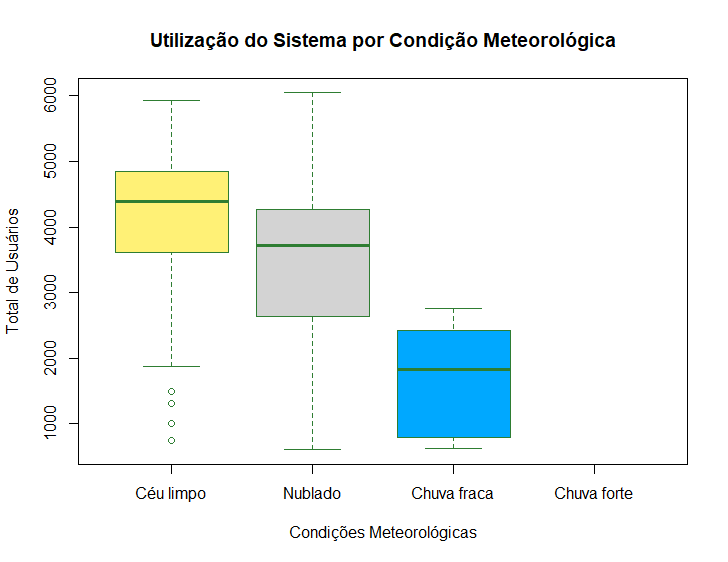
\includegraphics[width=0.6\textwidth]{Boxplot_clima.png}
    \caption{Boxplot do total de usuários por condição meteorológica}
    \label{fig:boxplot_clima}
\end{figure}

Os resultados indicam que a demanda pelo sistema cai de forma expressiva à medida que as condições meteorológicas se deterioram. A média de usuários cai de cerca de 4159, em dias de céu limpo, para apenas 1757, em dias de chuva fraca, o que corresponde a quase 2/3 a menos de usuários do sistema em dias de chuva fraca em comparação com o céu limpo, o que se nota graficamente pela queda em \textquotedblleft degraus\textquotedblright{} das medianas representadas no boxplot. Além disso, observa-se uma imprevisibilidade no uso do sistema em dias nublados, tanto pelo maior desvio padrão quanto pelo tamanho da caixa e dos bigodes no boxplot, mostrando que, mesmo com o clima nublado, há dias de uso bastante elevado do sistema, enquanto outros igualam o nível de uso em dias chuvosos, denotando a clara variabilidade no comportamento dos usuários frente a essa condição climática.

% ==========================================
% 3.3 Item 3
% ==========================================

\subsection*{Item 3}
\addcontentsline{toc}{subsection}{Item 3}
Este item busca investigar a relação entre temperatura e \texttt{total\_user}, usando para isso um gráfico de dispersão e o coeficiente de correlação para descrever a relação observada. Para isso, foi utilizado o seguinte código em R:

% ----------- Código 14 -------------
\begin{rcode}[firstnumber=155, caption={Obtenção do coeficiente de correlação de Pearson e plotagem do gráfico de dispersão},breaklines=true, breakatwhitespace=true]
    #item 3
    # Cálculo do coeficiente de correlação de Pearson
    correlacao <- cor(data_group$temp, total_user)
    print(correlacao)

    # Construção do gráfico de dispersão
    plot(data_group$temp, total_user,
        main = "Relação entre temperatura e utilização do sistema",
        xlab = "Temperatura em graus Celsius",
        ylab = "Total de Usuários",
        pch = 19,               # Formato do ponto (bolinha preenchida)
        col = "#2E7D32",        # Cor dos pontos
        frame.plot = FALSE)     # Remove a moldura externa superior e direita
\end{rcode}

Primeiro é extraído diretamente o coeficiente de correlação (que no R, por padrão, é o de Pearson) através da função \texttt{cor(data\_group\$temp, total\_user)}, correlacionando a temperatura e o \texttt{total\_user}.

O resultado obtido no terminal foi $r = 0.6386851$, o que denota uma correlação positiva e moderada-alta, ainda distante de 1, o que indica que, com o aumento da temperatura, o número de usuários do sistema tende a aumentar, entretanto com uma considerável dispersão dos pontos no gráfico, indicando que outros fatores também influenciam nessa relação.

% ------------ Imagem 5 -----------
\begin{figure}[htbp]
    \centering
    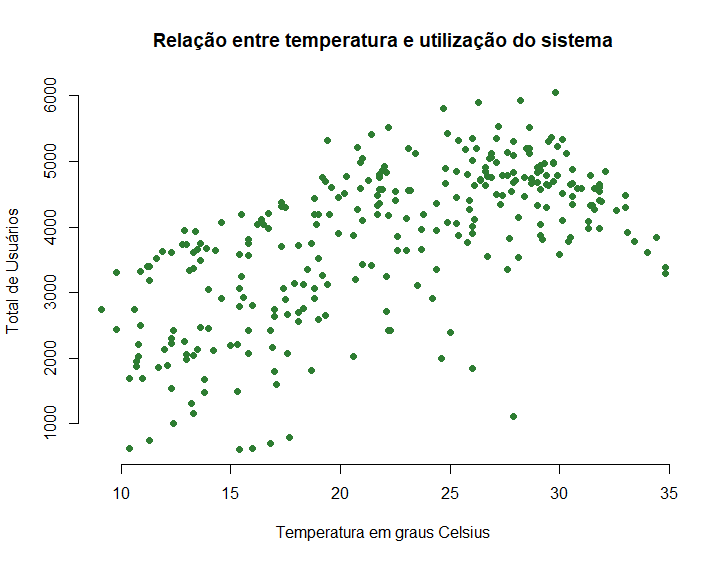
\includegraphics[width=0.55\textwidth]{Dispersao_temp.png}
    \caption{Gráfico de dispersão (\texttt{total\_user} x temperatura)}
    \label{fig:dispersao_temp}
\end{figure}

Evidenciam-se, portanto, algumas limitações do coeficiente de Pearson para descrever essa relação. Por exemplo, o $r$ de Pearson é estritamente linear, o que reduz sua precisão em relações não lineares: nota-se um crescimento quase linear até por volta dos 30°C, e depois disso o total de usuários começa a cair com o aumento da temperatura, o que formaria uma curva em parábola, relação que o coeficiente linear não captura. Além disso, por natureza, correlação não implica causalidade, e também é sensível a outliers, como pontos isolados de baixo uso do sistema bem abaixo do padrão da vizinhança, que tende a ser mais alto.

% ==========================================
% 3.4 Item 4
% ==========================================

\subsection*{Item 4}
\addcontentsline{toc}{subsection}{Item 4}
Este item pede para escolher 2 das 3 categorias analisadas previamente nesta questão que parecem estar mais associadas à utilização do sistema. Baseado nos dados obtidos e na análise feita, as duas categorias escolhidas serão a condição meteorológica e a temperatura, pois, apesar da estação do ano influenciar a demanda do sistema, ela é uma categoria que engloba em partes características das outras duas. Por exemplo, no item 1 observou-se que, no inverno, a demanda pelo sistema cai consideravelmente; entretanto, o inverno afasta as pessoas justamente pelo fato de ter temperaturas baixas e condições meteorológicas mais turbulentas, e nos itens 2 e 3 foi comprovado que condições meteorológicas piores e temperaturas baixas têm, no geral, baixa adesão dos usuários ao sistema. Feita essa escolha das 2 categorias, os resultados estatísticos mostram o seguinte sobre elas:

\textit{Condições meteorológicas:}

Observou-se que esta categoria é um fator altamente impactante na demanda do sistema, visto que a média de usuários despencou de 4159, em dias de céu limpo, para somente 1757, em dias de chuva fraca. Além disso, através da análise da proporção de dias classificados como \texttt{low\_usage}, 100\% dos dias com chuva fraca registraram baixa utilização do sistema, provando ser um fator drástico que limita a quantidade de usuários que aderem ao sistema de aluguel de bicicletas, sendo assim uma categoria intensamente associada à utilização do sistema.

\textit{Temperatura:}

Os resultados mostram que a temperatura possui considerável relação com a utilização do sistema. Através do coeficiente de correlação de Pearson obtido ($r \approx 0.64$), evidencia-se uma forte associação linear positiva, com o gráfico de dispersão ilustrando claramente o aumento gradual no número de usuários conforme a temperatura aumenta, até um limite de conforto e saúde por volta de 30-32°C. Além disso, o gráfico de dispersão, apesar de estar analisando a relação temperatura x total de usuários, também reforça a associação encontrada no item 1 entre estação do ano e \texttt{total\_user}, constatando-se que estações do ano mais frias apresentam médias de usuários menores do que estações mais quentes, com a média de usuários do inverno (2000) sendo menos da metade da média de usuários do verão (4464).
)
% ==========================================

A questão 3 solicita o uso da variável \texttt{low\_usage} previamente definida na questão 2 para investigar as características associadas aos dias de menor uso do sistema.

% ==========================================
% 3.0 Definições
% ==========================================

\subsection*{Definições}
\addcontentsline{toc}{subsection}{Definições}
\noindent \textit{def} - Desvio padrão: indica o quão espalhados estão os valores de um conjunto de dados em relação à média, utilizado aqui como desvio padrão amostral, já que estamos analisando uma amostra de 300 valores de uma população total de 731. O desvio padrão amostral é o mesmo utilizado pela função \texttt{sd()} do R, dado pela fórmula:

\begin{equation*}
    s = \sqrt{\frac{1}{N-1}\sum_{i=1}^{N}\left(x_i-\overline{x}\right)^2}
\end{equation*}

\noindent \textit{def} - Coeficiente de correlação de Pearson: mede a intensidade da relação linear entre duas variáveis quantitativas, retornando um valor entre $-1$ e $1$, dado pela fórmula:

\begin{equation*}
    r = \frac{\sum\left(x_i-\overline{x}\right)\left(y_i-\overline{y}\right)}{\sqrt{\sum\left(x_i-\overline{x}\right)^2\sum\left(y_i-\overline{y}\right)^2}}
\end{equation*}

% ==========================================
% 3.1 Item 1
% ==========================================

\subsection*{Item 1}
\addcontentsline{toc}{subsection}{Item 1}
Este item pede para calcular média, mediana e desvio padrão de \texttt{total\_user} para cada estação do ano e determinar a proporção de dias classificados como \texttt{low\_usage} e, além disso, construir um boxplot comparando cada estação.

Para a resolução do item 1, segue o código em R e a explicação de cada trecho:

% ----------- Código 11 -------------
\begin{rcode}[firstnumber=109, caption={Análise da utilização do sistema em cada estação do ano},breaklines=true, breakatwhitespace=true]
    # Questão 3
    # Item 1
    # Convertendo season numérico para categórico
    data_group$season <- factor(data_group$season,
                                levels = c(1, 2, 3, 4),
                                labels = c("Inverno", "Primavera", "Verão", "Outono"))
    # Média de usuários por estação do ano
    tapply(total_user, data_group$season, mean)
    # Mediana de usuários por estação
    tapply(total_user, data_group$season, median)
    # Desvio padrão de total_user por estação
    tapply(total_user, data_group$season, sd)
    # Proporção de dias classificados como low_usage por estação
    tapply(low_usage, data_group$season, mean)

    boxplot(total_user ~ data_group$season,
            main = "Comparação do uso do sistema por Estação", #Titulo
            xlab = "Estação do Ano", #legenda eixo x
            ylab = "Total de Usuários", #legenda eixo y
            medcol = "#D32F2F",        # Cor da mediana
            col = c("#81C784", "#FFF176", "#FFB74D", "#64B5F6"), #cores das caixas
            border = "#2E7D32") #cor da borda da caixa
\end{rcode}

Primeiro é feita a conversão da variável \texttt{season} de numérica para categórica usando \texttt{factor} para associar o nome de cada estação ao seu respectivo número (1, 2, 3, 4). A conversão não altera os valores calculados, apenas faz com que os grupos sejam identificados pelo nome da estação, tanto na saída da função \texttt{tapply} quanto no eixo do boxplot. Depois, é utilizada a função \texttt{tapply()} para dividir o vetor de \texttt{total\_user} em subgrupos, um para cada estação do ano, e aplicar uma função (no caso aqui, as funções de média, mediana e desvio padrão) a cada subgrupo deste vetor. O resultado obtido no R está na tabela a seguir:

% ----------- Tabela 7  -------------
\begin{table}[h!]
    \centering
    \caption{Resultados para cada estação}
    \label{tab:mascara_7u}
    \begin{tabular}{c|c|c|c|c}
        Medição & Inverno & Primavera & Verão & Outono \\\hline
        Média &2000.76 &3775.17 &4464.36 &3664.46 \\ \hline
        Mediana &2077.00 &4085.50 &4615.50 &3717.00 \\ \hline
        Desvio padrão &738.80 &1138.90 &798.35 &983.01 \\ \hline
        Proporção (\texttt{low\_usage}) &0.92 &0.26 &0.04 &0.27
    \end{tabular}
\end{table}

Como a variável \texttt{low\_usage} é 0 ou 1, fazer a média retorna exatamente a proporção, já que estamos somando os dias classificados como \texttt{low\_usage} e dividindo pela quantidade de dias.

Para a construção do boxplot, foi feita a criação do gráfico fazendo:
\begin{center}
    \texttt{total\_user \textasciitilde{} data\_group\$season}
\end{center}
Ou seja, \texttt{total\_user} em função da variável \texttt{season}, gerando uma caixa para cada estação. O boxplot gerado está exibido a seguir:

% ------------ Imagem 3 -----------
\begin{figure}[htbp]
    \centering
    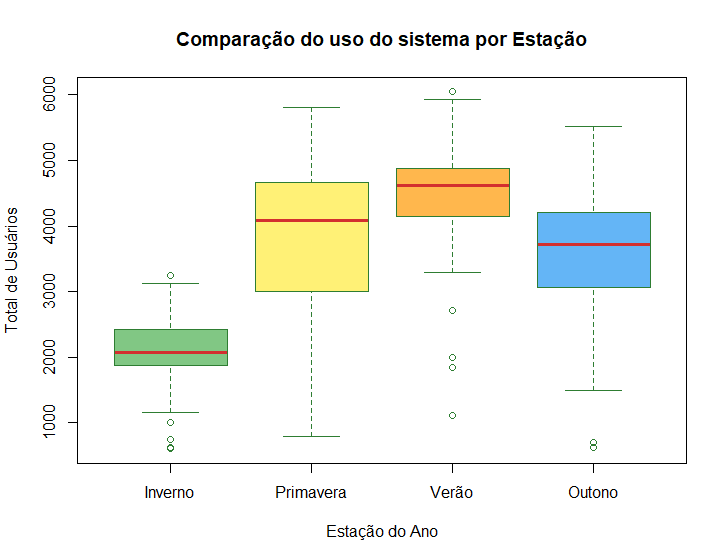
\includegraphics[width=0.6\textwidth]{Boxplot_estacoes.png}
    \caption{Boxplot do total de usuários por estação}
    \label{fig:boxplot_estacoes}
\end{figure}

Os resultados evidenciam uma clara associação entre as estações do ano e o uso do sistema, mostrando que o uso diminui consideravelmente no período de inverno e aumenta nas estações mais quentes. Além disso, a extração da proporção de dias classificados como \texttt{low\_usage} denota que a grande maioria dos dias de inverno é classificada como de baixa utilização do sistema, ademais, o uso do sistema no verão aumenta mais que o dobro do que no inverno, com o verão tendo uma média total de usuários do sistema de 4464.36 contra uma média de 2000.76 usuários no inverno. Outra informação relevante é que as estações de primavera e outono possuem média de usuários diária bem próxima, o que demonstra que o uso do sistema é bem equivalente entre essas duas estações, com uma ressalva de que a primavera tem alto desvio padrão comparado às outras estações, evidenciando uma notável disparidade entre dias de maior uso e de menor uso dentro da própria estação devido a fatores além da estação do ano.

% ==========================================
% 3.2 Item 2
% ==========================================

\subsection*{Item 2}
\addcontentsline{toc}{subsection}{Item 2}
Este item busca investigar a relação do uso do sistema em função das condições meteorológicas. Para isso, o item pede que, para cada condição, seja calculada a média e o desvio padrão de \texttt{total\_user} e determinada a proporção de dias classificados como \texttt{low\_usage}.

Para isso, foi utilizado o seguinte código em R:

% ----------- Código 12 -------------
\begin{rcode}[firstnumber=132, caption={Análise da utilização do sistema para cada condição meteorológica},breaklines=true, breakatwhitespace=true]
    # Item 2
    # Convertendo weathersit de numérico para categórico
    data_group$weathersit <- factor(data_group$weathersit,
                                    levels = c(1, 2, 3, 4),
                                    labels = c("Céu limpo", "Nublado", "Chuva fraca", "Chuva forte"))

    # Média total_user por condição meteorológica
    tapply(total_user, data_group$weathersit, mean)

    # Desvio padrão de total_user por condição meteorológica
    tapply(total_user, data_group$weathersit, sd)

    # Proporção de dias de baixa utilização (low_usage) por condição meteorológica
    tapply(low_usage, data_group$weathersit, mean)
\end{rcode}

Assim como na resolução do item 1, foi utilizada a seguinte linha de raciocínio: para cada valor correspondente a determinada condição climática constatada no \texttt{data\_group}, foi associado o nome correspondente da condição climática utilizando \texttt{factor}, para facilitar a identificação e interpretação dos dados tanto nos resultados da função \texttt{tapply} quanto em representações gráficas. Após isso, usando a função \texttt{tapply} para aplicar as funções de média e desvio padrão a cada subgrupo de \texttt{total\_user} e de \texttt{low\_usage} (um para cada condição meteorológica), obtiveram-se os seguintes resultados de média, desvio padrão e proporção de dias classificados como baixo uso do sistema, constatados na tabela a seguir:

% ----------- Tabela 8  -------------
\begin{table}[h!]
    \centering
    \caption{Resultados para cada condição meteorológica}
    \label{tab:mascara_8u}
    \begin{tabular}{c|c|c|c|c}
        Medição & Céu limpo & Nublado & Chuva fraca & Chuva forte \\\hline
        Média &4159.22 &3462.94 &1757.57 &-- \\ \hline
        Desvio padrão &984.66 &1090.92 &793.95 &-- \\ \hline
        Proporção (\texttt{low\_usage}) &0.14 &0.35 &1.00 &--
    \end{tabular}
\end{table}

Analisando os resultados, nota-se de imediato duas informações cruciais: não se obtiveram dados para a categoria de chuva forte, pois o \texttt{data\_group} de 300 amostras não possui dias classificados meteorologicamente com essa condição climática; além disso, destaca-se a proporção de dias de baixo uso igual a 1, ou seja, nos dias de chuva fraca da amostra, o total de usuários ficou sempre abaixo do primeiro quartil (Q1) definido para a amostra inteira.

Para realizar uma comparação visual entre as condições meteorológicas, usou-se também um gráfico construído a partir do seguinte código em R:

% ----------- Código 13 -------------
\begin{rcode}[firstnumber=147, caption={Construção de boxplot para análise da utilização do sistema para cada condição meteorológica},breaklines=true, breakatwhitespace=true]
    # Boxplot
    boxplot(total_user ~ data_group$weathersit,
            main = "Utilização do Sistema por Condição Meteorológica",
            xlab = "Condições Meteorológicas",
            ylab = "Total de Usuários",
            col = c("#FFF176", "#D3D3D3", "#00A8FF", "#173A59"),
            border = "#2E7D32")
\end{rcode}

% ------------ Imagem 4 -----------
\begin{figure}[htbp]
    \centering
    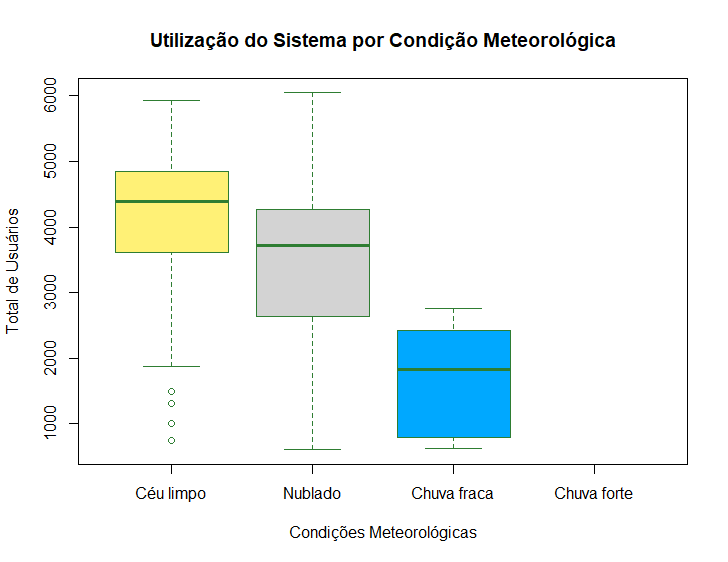
\includegraphics[width=0.6\textwidth]{Boxplot_clima.png}
    \caption{Boxplot do total de usuários por condição meteorológica}
    \label{fig:boxplot_clima}
\end{figure}

Os resultados indicam que a demanda pelo sistema cai de forma expressiva à medida que as condições meteorológicas se deterioram. A média de usuários cai de cerca de 4159, em dias de céu limpo, para apenas 1757, em dias de chuva fraca, o que corresponde a quase 2/3 a menos de usuários do sistema em dias de chuva fraca em comparação com o céu limpo, o que se nota graficamente pela queda em \textquotedblleft degraus\textquotedblright{} das medianas representadas no boxplot. Além disso, observa-se uma imprevisibilidade no uso do sistema em dias nublados, tanto pelo maior desvio padrão quanto pelo tamanho da caixa e dos bigodes no boxplot, mostrando que, mesmo com o clima nublado, há dias de uso bastante elevado do sistema, enquanto outros igualam o nível de uso em dias chuvosos, denotando a clara variabilidade no comportamento dos usuários frente a essa condição climática.

% ==========================================
% 3.3 Item 3
% ==========================================

\subsection*{Item 3}
\addcontentsline{toc}{subsection}{Item 3}
Este item busca investigar a relação entre temperatura e \texttt{total\_user}, usando para isso um gráfico de dispersão e o coeficiente de correlação para descrever a relação observada. Para isso, foi utilizado o seguinte código em R:

% ----------- Código 14 -------------
\begin{rcode}[firstnumber=155, caption={Obtenção do coeficiente de correlação de Pearson e plotagem do gráfico de dispersão},breaklines=true, breakatwhitespace=true]
    #item 3
    # Cálculo do coeficiente de correlação de Pearson
    correlacao <- cor(data_group$temp, total_user)
    print(correlacao)

    # Construção do gráfico de dispersão
    plot(data_group$temp, total_user,
        main = "Relação entre temperatura e utilização do sistema",
        xlab = "Temperatura em graus Celsius",
        ylab = "Total de Usuários",
        pch = 19,               # Formato do ponto (bolinha preenchida)
        col = "#2E7D32",        # Cor dos pontos
        frame.plot = FALSE)     # Remove a moldura externa superior e direita
\end{rcode}

Primeiro é extraído diretamente o coeficiente de correlação (que no R, por padrão, é o de Pearson) através da função \texttt{cor(data\_group\$temp, total\_user)}, correlacionando a temperatura e o \texttt{total\_user}.

O resultado obtido no terminal foi $r = 0.6386851$, o que denota uma correlação positiva e moderada-alta, ainda distante de 1, o que indica que, com o aumento da temperatura, o número de usuários do sistema tende a aumentar, entretanto com uma considerável dispersão dos pontos no gráfico, indicando que outros fatores também influenciam nessa relação.

% ------------ Imagem 5 -----------
\begin{figure}[htbp]
    \centering
    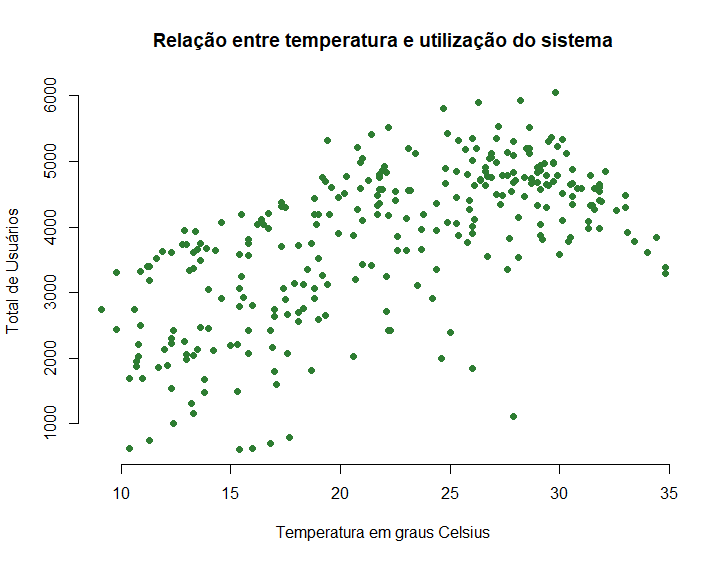
\includegraphics[width=0.55\textwidth]{Dispersao_temp.png}
    \caption{Gráfico de dispersão (\texttt{total\_user} x temperatura)}
    \label{fig:dispersao_temp}
\end{figure}

Evidenciam-se, portanto, algumas limitações do coeficiente de Pearson para descrever essa relação. Por exemplo, o $r$ de Pearson é estritamente linear, o que reduz sua precisão em relações não lineares: nota-se um crescimento quase linear até por volta dos 30°C, e depois disso o total de usuários começa a cair com o aumento da temperatura, o que formaria uma curva em parábola, relação que o coeficiente linear não captura. Além disso, por natureza, correlação não implica causalidade, e também é sensível a outliers, como pontos isolados de baixo uso do sistema bem abaixo do padrão da vizinhança, que tende a ser mais alto.

% ==========================================
% 3.4 Item 4
% ==========================================

\subsection*{Item 4}
\addcontentsline{toc}{subsection}{Item 4}
Este item pede para escolher 2 das 3 categorias analisadas previamente nesta questão que parecem estar mais associadas à utilização do sistema. Baseado nos dados obtidos e na análise feita, as duas categorias escolhidas serão a condição meteorológica e a temperatura, pois, apesar da estação do ano influenciar a demanda do sistema, ela é uma categoria que engloba em partes características das outras duas. Por exemplo, no item 1 observou-se que, no inverno, a demanda pelo sistema cai consideravelmente; entretanto, o inverno afasta as pessoas justamente pelo fato de ter temperaturas baixas e condições meteorológicas mais turbulentas, e nos itens 2 e 3 foi comprovado que condições meteorológicas piores e temperaturas baixas têm, no geral, baixa adesão dos usuários ao sistema. Feita essa escolha das 2 categorias, os resultados estatísticos mostram o seguinte sobre elas:

\textit{Condições meteorológicas:}

Observou-se que esta categoria é um fator altamente impactante na demanda do sistema, visto que a média de usuários despencou de 4159, em dias de céu limpo, para somente 1757, em dias de chuva fraca. Além disso, através da análise da proporção de dias classificados como \texttt{low\_usage}, 100\% dos dias com chuva fraca registraram baixa utilização do sistema, provando ser um fator drástico que limita a quantidade de usuários que aderem ao sistema de aluguel de bicicletas, sendo assim uma categoria intensamente associada à utilização do sistema.

\textit{Temperatura:}

Os resultados mostram que a temperatura possui considerável relação com a utilização do sistema. Através do coeficiente de correlação de Pearson obtido ($r \approx 0.64$), evidencia-se uma forte associação linear positiva, com o gráfico de dispersão ilustrando claramente o aumento gradual no número de usuários conforme a temperatura aumenta, até um limite de conforto e saúde por volta de 30-32°C. Além disso, o gráfico de dispersão, apesar de estar analisando a relação temperatura x total de usuários, também reforça a associação encontrada no item 1 entre estação do ano e \texttt{total\_user}, constatando-se que estações do ano mais frias apresentam médias de usuários menores do que estações mais quentes, com a média de usuários do inverno (2000) sendo menos da metade da média de usuários do verão (4464).
)
% ==========================================

A questão 3 solicita o uso da variável \texttt{low\_usage} previamente definida na questão 2 para investigar as características associadas aos dias de menor uso do sistema.

% ==========================================
% 3.0 Definições
% ==========================================

\subsection*{Definições}
\addcontentsline{toc}{subsection}{Definições}
\noindent \textit{def} - Desvio padrão: indica o quão espalhados estão os valores de um conjunto de dados em relação à média, utilizado aqui como desvio padrão amostral, já que estamos analisando uma amostra de 300 valores de uma população total de 731. O desvio padrão amostral é o mesmo utilizado pela função \texttt{sd()} do R, dado pela fórmula:

\begin{equation*}
    s = \sqrt{\frac{1}{N-1}\sum_{i=1}^{N}\left(x_i-\overline{x}\right)^2}
\end{equation*}

\noindent \textit{def} - Coeficiente de correlação de Pearson: mede a intensidade da relação linear entre duas variáveis quantitativas, retornando um valor entre $-1$ e $1$, dado pela fórmula:

\begin{equation*}
    r = \frac{\sum\left(x_i-\overline{x}\right)\left(y_i-\overline{y}\right)}{\sqrt{\sum\left(x_i-\overline{x}\right)^2\sum\left(y_i-\overline{y}\right)^2}}
\end{equation*}

% ==========================================
% 3.1 Item 1
% ==========================================

\subsection*{Item 1}
\addcontentsline{toc}{subsection}{Item 1}
Este item pede para calcular média, mediana e desvio padrão de \texttt{total\_user} para cada estação do ano e determinar a proporção de dias classificados como \texttt{low\_usage} e, além disso, construir um boxplot comparando cada estação.

Para a resolução do item 1, segue o código em R e a explicação de cada trecho:

% ----------- Código 11 -------------
\begin{rcode}[firstnumber=109, caption={Análise da utilização do sistema em cada estação do ano},breaklines=true, breakatwhitespace=true]
    # Questão 3
    # Item 1
    # Convertendo season numérico para categórico
    data_group$season <- factor(data_group$season,
                                levels = c(1, 2, 3, 4),
                                labels = c("Inverno", "Primavera", "Verão", "Outono"))
    # Média de usuários por estação do ano
    tapply(total_user, data_group$season, mean)
    # Mediana de usuários por estação
    tapply(total_user, data_group$season, median)
    # Desvio padrão de total_user por estação
    tapply(total_user, data_group$season, sd)
    # Proporção de dias classificados como low_usage por estação
    tapply(low_usage, data_group$season, mean)

    boxplot(total_user ~ data_group$season,
            main = "Comparação do uso do sistema por Estação", #Titulo
            xlab = "Estação do Ano", #legenda eixo x
            ylab = "Total de Usuários", #legenda eixo y
            medcol = "#D32F2F",        # Cor da mediana
            col = c("#81C784", "#FFF176", "#FFB74D", "#64B5F6"), #cores das caixas
            border = "#2E7D32") #cor da borda da caixa
\end{rcode}

Primeiro é feita a conversão da variável \texttt{season} de numérica para categórica usando \texttt{factor} para associar o nome de cada estação ao seu respectivo número (1, 2, 3, 4). A conversão não altera os valores calculados, apenas faz com que os grupos sejam identificados pelo nome da estação, tanto na saída da função \texttt{tapply} quanto no eixo do boxplot. Depois, é utilizada a função \texttt{tapply()} para dividir o vetor de \texttt{total\_user} em subgrupos, um para cada estação do ano, e aplicar uma função (no caso aqui, as funções de média, mediana e desvio padrão) a cada subgrupo deste vetor. O resultado obtido no R está na tabela a seguir:

% ----------- Tabela 7  -------------
\begin{table}[h!]
    \centering
    \caption{Resultados para cada estação}
    \label{tab:mascara_7u}
    \begin{tabular}{c|c|c|c|c}
        Medição & Inverno & Primavera & Verão & Outono \\\hline
        Média &2000.76 &3775.17 &4464.36 &3664.46 \\ \hline
        Mediana &2077.00 &4085.50 &4615.50 &3717.00 \\ \hline
        Desvio padrão &738.80 &1138.90 &798.35 &983.01 \\ \hline
        Proporção (\texttt{low\_usage}) &0.92 &0.26 &0.04 &0.27
    \end{tabular}
\end{table}

Como a variável \texttt{low\_usage} é 0 ou 1, fazer a média retorna exatamente a proporção, já que estamos somando os dias classificados como \texttt{low\_usage} e dividindo pela quantidade de dias.

Para a construção do boxplot, foi feita a criação do gráfico fazendo:
\begin{center}
    \texttt{total\_user \textasciitilde{} data\_group\$season}
\end{center}
Ou seja, \texttt{total\_user} em função da variável \texttt{season}, gerando uma caixa para cada estação. O boxplot gerado está exibido a seguir:

% ------------ Imagem 3 -----------
\begin{figure}[htbp]
    \centering
    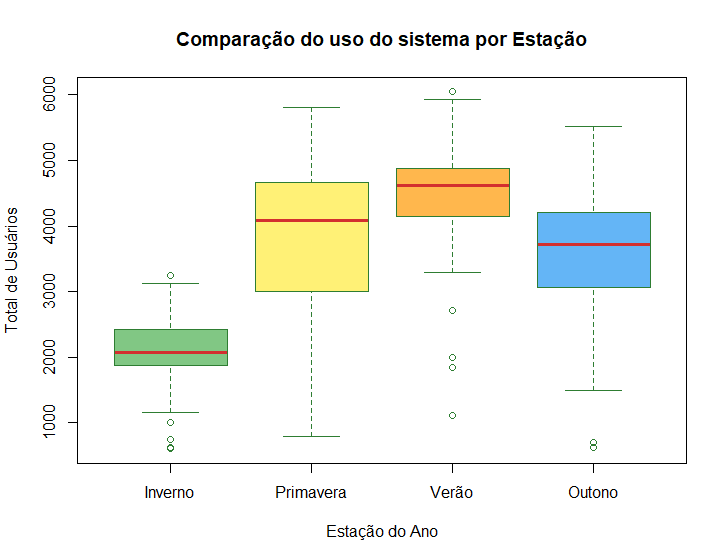
\includegraphics[width=0.6\textwidth]{Boxplot_estacoes.png}
    \caption{Boxplot do total de usuários por estação}
    \label{fig:boxplot_estacoes}
\end{figure}

Os resultados evidenciam uma clara associação entre as estações do ano e o uso do sistema, mostrando que o uso diminui consideravelmente no período de inverno e aumenta nas estações mais quentes. Além disso, a extração da proporção de dias classificados como \texttt{low\_usage} denota que a grande maioria dos dias de inverno é classificada como de baixa utilização do sistema, ademais, o uso do sistema no verão aumenta mais que o dobro do que no inverno, com o verão tendo uma média total de usuários do sistema de 4464.36 contra uma média de 2000.76 usuários no inverno. Outra informação relevante é que as estações de primavera e outono possuem média de usuários diária bem próxima, o que demonstra que o uso do sistema é bem equivalente entre essas duas estações, com uma ressalva de que a primavera tem alto desvio padrão comparado às outras estações, evidenciando uma notável disparidade entre dias de maior uso e de menor uso dentro da própria estação devido a fatores além da estação do ano.

% ==========================================
% 3.2 Item 2
% ==========================================

\subsection*{Item 2}
\addcontentsline{toc}{subsection}{Item 2}
Este item busca investigar a relação do uso do sistema em função das condições meteorológicas. Para isso, o item pede que, para cada condição, seja calculada a média e o desvio padrão de \texttt{total\_user} e determinada a proporção de dias classificados como \texttt{low\_usage}.

Para isso, foi utilizado o seguinte código em R:

% ----------- Código 12 -------------
\begin{rcode}[firstnumber=132, caption={Análise da utilização do sistema para cada condição meteorológica},breaklines=true, breakatwhitespace=true]
    # Item 2
    # Convertendo weathersit de numérico para categórico
    data_group$weathersit <- factor(data_group$weathersit,
                                    levels = c(1, 2, 3, 4),
                                    labels = c("Céu limpo", "Nublado", "Chuva fraca", "Chuva forte"))

    # Média total_user por condição meteorológica
    tapply(total_user, data_group$weathersit, mean)

    # Desvio padrão de total_user por condição meteorológica
    tapply(total_user, data_group$weathersit, sd)

    # Proporção de dias de baixa utilização (low_usage) por condição meteorológica
    tapply(low_usage, data_group$weathersit, mean)
\end{rcode}

Assim como na resolução do item 1, foi utilizada a seguinte linha de raciocínio: para cada valor correspondente a determinada condição climática constatada no \texttt{data\_group}, foi associado o nome correspondente da condição climática utilizando \texttt{factor}, para facilitar a identificação e interpretação dos dados tanto nos resultados da função \texttt{tapply} quanto em representações gráficas. Após isso, usando a função \texttt{tapply} para aplicar as funções de média e desvio padrão a cada subgrupo de \texttt{total\_user} e de \texttt{low\_usage} (um para cada condição meteorológica), obtiveram-se os seguintes resultados de média, desvio padrão e proporção de dias classificados como baixo uso do sistema, constatados na tabela a seguir:

% ----------- Tabela 8  -------------
\begin{table}[h!]
    \centering
    \caption{Resultados para cada condição meteorológica}
    \label{tab:mascara_8u}
    \begin{tabular}{c|c|c|c|c}
        Medição & Céu limpo & Nublado & Chuva fraca & Chuva forte \\\hline
        Média &4159.22 &3462.94 &1757.57 &-- \\ \hline
        Desvio padrão &984.66 &1090.92 &793.95 &-- \\ \hline
        Proporção (\texttt{low\_usage}) &0.14 &0.35 &1.00 &--
    \end{tabular}
\end{table}

Analisando os resultados, nota-se de imediato duas informações cruciais: não se obtiveram dados para a categoria de chuva forte, pois o \texttt{data\_group} de 300 amostras não possui dias classificados meteorologicamente com essa condição climática; além disso, destaca-se a proporção de dias de baixo uso igual a 1, ou seja, nos dias de chuva fraca da amostra, o total de usuários ficou sempre abaixo do primeiro quartil (Q1) definido para a amostra inteira.

Para realizar uma comparação visual entre as condições meteorológicas, usou-se também um gráfico construído a partir do seguinte código em R:

% ----------- Código 13 -------------
\begin{rcode}[firstnumber=147, caption={Construção de boxplot para análise da utilização do sistema para cada condição meteorológica},breaklines=true, breakatwhitespace=true]
    # Boxplot
    boxplot(total_user ~ data_group$weathersit,
            main = "Utilização do Sistema por Condição Meteorológica",
            xlab = "Condições Meteorológicas",
            ylab = "Total de Usuários",
            col = c("#FFF176", "#D3D3D3", "#00A8FF", "#173A59"),
            border = "#2E7D32")
\end{rcode}

% ------------ Imagem 4 -----------
\begin{figure}[htbp]
    \centering
    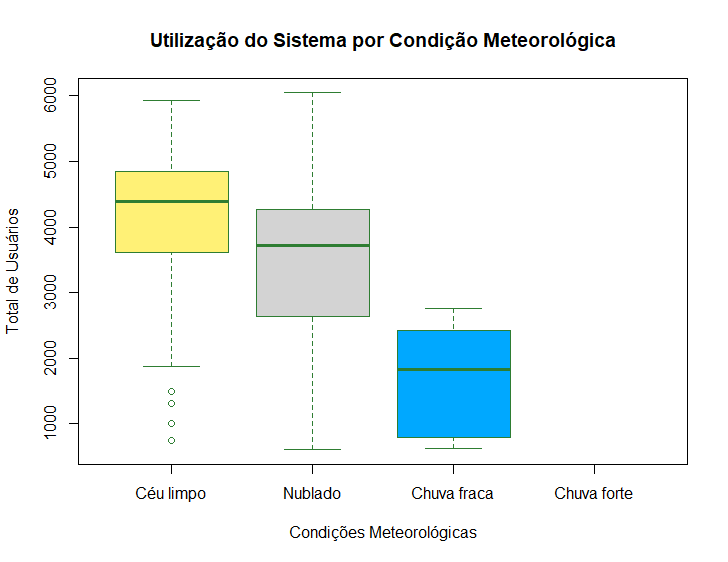
\includegraphics[width=0.6\textwidth]{Boxplot_clima.png}
    \caption{Boxplot do total de usuários por condição meteorológica}
    \label{fig:boxplot_clima}
\end{figure}

Os resultados indicam que a demanda pelo sistema cai de forma expressiva à medida que as condições meteorológicas se deterioram. A média de usuários cai de cerca de 4159, em dias de céu limpo, para apenas 1757, em dias de chuva fraca, o que corresponde a quase 2/3 a menos de usuários do sistema em dias de chuva fraca em comparação com o céu limpo, o que se nota graficamente pela queda em \textquotedblleft degraus\textquotedblright{} das medianas representadas no boxplot. Além disso, observa-se uma imprevisibilidade no uso do sistema em dias nublados, tanto pelo maior desvio padrão quanto pelo tamanho da caixa e dos bigodes no boxplot, mostrando que, mesmo com o clima nublado, há dias de uso bastante elevado do sistema, enquanto outros igualam o nível de uso em dias chuvosos, denotando a clara variabilidade no comportamento dos usuários frente a essa condição climática.

% ==========================================
% 3.3 Item 3
% ==========================================

\subsection*{Item 3}
\addcontentsline{toc}{subsection}{Item 3}
Este item busca investigar a relação entre temperatura e \texttt{total\_user}, usando para isso um gráfico de dispersão e o coeficiente de correlação para descrever a relação observada. Para isso, foi utilizado o seguinte código em R:

% ----------- Código 14 -------------
\begin{rcode}[firstnumber=155, caption={Obtenção do coeficiente de correlação de Pearson e plotagem do gráfico de dispersão},breaklines=true, breakatwhitespace=true]
    #item 3
    # Cálculo do coeficiente de correlação de Pearson
    correlacao <- cor(data_group$temp, total_user)
    print(correlacao)

    # Construção do gráfico de dispersão
    plot(data_group$temp, total_user,
        main = "Relação entre temperatura e utilização do sistema",
        xlab = "Temperatura em graus Celsius",
        ylab = "Total de Usuários",
        pch = 19,               # Formato do ponto (bolinha preenchida)
        col = "#2E7D32",        # Cor dos pontos
        frame.plot = FALSE)     # Remove a moldura externa superior e direita
\end{rcode}

Primeiro é extraído diretamente o coeficiente de correlação (que no R, por padrão, é o de Pearson) através da função \texttt{cor(data\_group\$temp, total\_user)}, correlacionando a temperatura e o \texttt{total\_user}.

O resultado obtido no terminal foi $r = 0.6386851$, o que denota uma correlação positiva e moderada-alta, ainda distante de 1, o que indica que, com o aumento da temperatura, o número de usuários do sistema tende a aumentar, entretanto com uma considerável dispersão dos pontos no gráfico, indicando que outros fatores também influenciam nessa relação.

% ------------ Imagem 5 -----------
\begin{figure}[htbp]
    \centering
    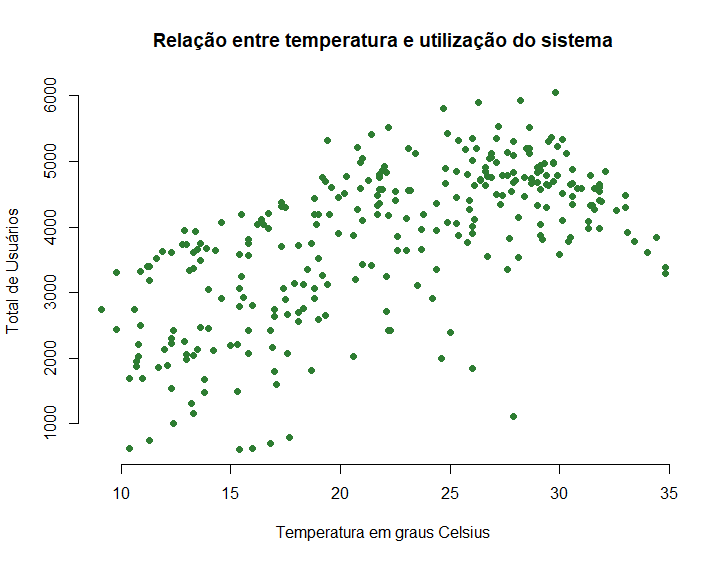
\includegraphics[width=0.55\textwidth]{Dispersao_temp.png}
    \caption{Gráfico de dispersão (\texttt{total\_user} x temperatura)}
    \label{fig:dispersao_temp}
\end{figure}

Evidenciam-se, portanto, algumas limitações do coeficiente de Pearson para descrever essa relação. Por exemplo, o $r$ de Pearson é estritamente linear, o que reduz sua precisão em relações não lineares: nota-se um crescimento quase linear até por volta dos 30°C, e depois disso o total de usuários começa a cair com o aumento da temperatura, o que formaria uma curva em parábola, relação que o coeficiente linear não captura. Além disso, por natureza, correlação não implica causalidade, e também é sensível a outliers, como pontos isolados de baixo uso do sistema bem abaixo do padrão da vizinhança, que tende a ser mais alto.

% ==========================================
% 3.4 Item 4
% ==========================================

\subsection*{Item 4}
\addcontentsline{toc}{subsection}{Item 4}
Este item pede para escolher 2 das 3 categorias analisadas previamente nesta questão que parecem estar mais associadas à utilização do sistema. Baseado nos dados obtidos e na análise feita, as duas categorias escolhidas serão a condição meteorológica e a temperatura, pois, apesar da estação do ano influenciar a demanda do sistema, ela é uma categoria que engloba em partes características das outras duas. Por exemplo, no item 1 observou-se que, no inverno, a demanda pelo sistema cai consideravelmente; entretanto, o inverno afasta as pessoas justamente pelo fato de ter temperaturas baixas e condições meteorológicas mais turbulentas, e nos itens 2 e 3 foi comprovado que condições meteorológicas piores e temperaturas baixas têm, no geral, baixa adesão dos usuários ao sistema. Feita essa escolha das 2 categorias, os resultados estatísticos mostram o seguinte sobre elas:

\textit{Condições meteorológicas:}

Observou-se que esta categoria é um fator altamente impactante na demanda do sistema, visto que a média de usuários despencou de 4159, em dias de céu limpo, para somente 1757, em dias de chuva fraca. Além disso, através da análise da proporção de dias classificados como \texttt{low\_usage}, 100\% dos dias com chuva fraca registraram baixa utilização do sistema, provando ser um fator drástico que limita a quantidade de usuários que aderem ao sistema de aluguel de bicicletas, sendo assim uma categoria intensamente associada à utilização do sistema.

\textit{Temperatura:}

Os resultados mostram que a temperatura possui considerável relação com a utilização do sistema. Através do coeficiente de correlação de Pearson obtido ($r \approx 0.64$), evidencia-se uma forte associação linear positiva, com o gráfico de dispersão ilustrando claramente o aumento gradual no número de usuários conforme a temperatura aumenta, até um limite de conforto e saúde por volta de 30-32°C. Além disso, o gráfico de dispersão, apesar de estar analisando a relação temperatura x total de usuários, também reforça a associação encontrada no item 1 entre estação do ano e \texttt{total\_user}, constatando-se que estações do ano mais frias apresentam médias de usuários menores do que estações mais quentes, com a média de usuários do inverno (2000) sendo menos da metade da média de usuários do verão (4464).
